\subsection{Historia}

Na początku XX wieku, gdy sieci telekomunikacyjne dopiero się rozwijały, wszystkie połączenia zestawiane były ręcznie. W momencie, gdy abonent podnosił słuchawkę telefonu, jego aparat wysyłał sygnał do lokalnej centrali telefonicznej. Na tablicy świetlnej zapalała się lampka informująca telefonistkę o próbie połączenia. Telefonistka odbierała, pytając, z kim abonent chce się połączyć. Następnie wprowadzała odpowiednią wtyczkę do odpowiedniego gniazda na tablicy rozdzielczej, zestawiając fizyczne połączenie między dwoma liniami. Jeśli rozmowa miała się odbyć na większą odległość (np. między miastami) połączenie przekazywane było przez kolejne centrale. Każda centrala po drodze wymagała ręcznej obsługi przez pracujące w nich telefonistki. 

\begin{figure}[!htbp]
    \centering 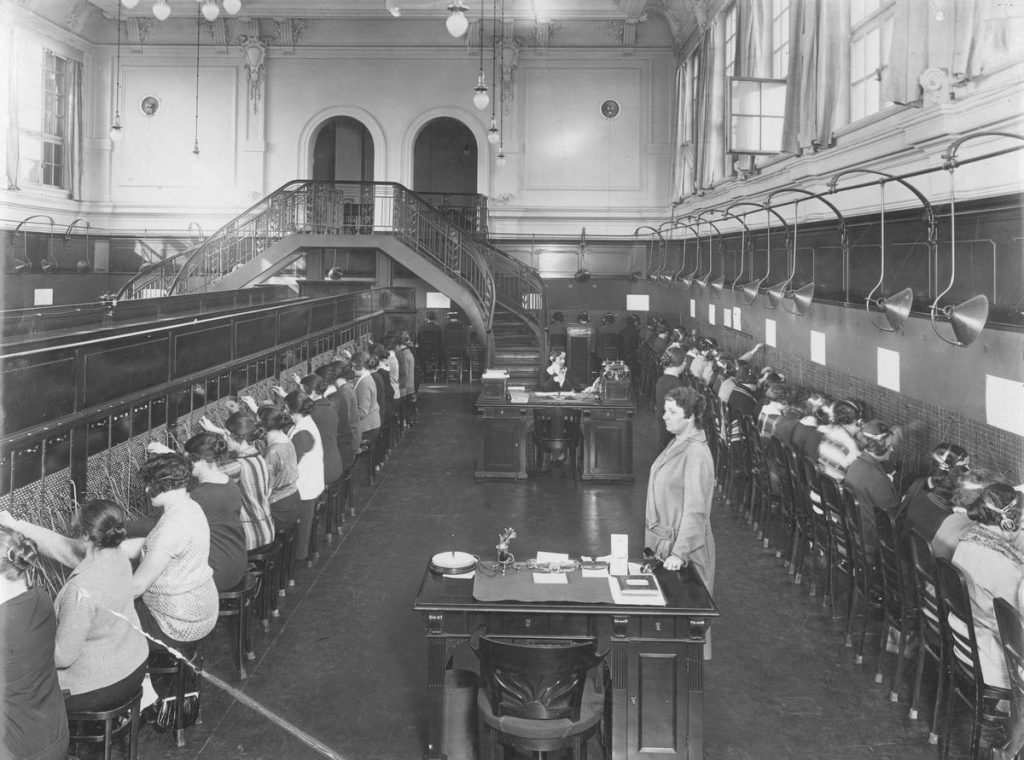
\includegraphics[width=1\linewidth]{telefonistki.jpg}
    \caption{Pracowniczki warszawskiej centrali telefonicznej z końca lat 20. XX wieku}\label{fig:telefonistki}
\end{figure}

Dziś taki scenariusz wydaje się wręcz absurdalny, a oferty pracy dla telefonistek dawno już zniknęły z tablic ogłoszeń. Praca wykonywana przez telefonistki (czyli komutacja łączy) nadal jest potrzebna do prawidłowego funkcjonowania sieci telekomunikacyjnych, lecz wykonywana jest przez programy komputerowe w sposób w pełni zautomatyzowany. Ręczna komutacja była pierwszym krokiem w kierunku rozwoju globalnych sieci telekomunikacyjnych i choć z dzisiejszej perspektywy wydaje się być bardzo pracochłonna i ograniczająca, bez niej nie powstałyby fundamenty, na których oparto późniejsze systemy automatyczne. Jest to przykład tego, jak technologia stopniowo uwalniała człowieka od bezpośredniej obsługi różnych systemów dając mu przestrzeń na rozwój w innych obszarach.

Na zasadzie indukcji możemy przyjąć, iż dziś znajdujemy się w podobnym położeniu - sieci telekomunikacyjne wciąż wymagają bezpośredniego zarządzania przez człowieka. Współcześnie granica styku - system-człowiek - jest mocno przesunięta, a interakcja zachodzi na dużo wyższym poziomie abstrakcji – zamiast fizycznie łączyć linie, operatorzy zarządzają skomplikowanymi systemami sterowania ruchem telekomunikacyjnym.. Możliwe, że nie istnieje ostateczny punkt styku i systemy telekomunikacyjne zawsze będą wymagały nadzoru ludzkiego. Niezależnie od tej kwestii przesunięcie wspomnianej granicy w czasach telefonistek, a dziś wymaga automatyzacji innego rodzaju. 

O telefonistkach możemy powiedzieć, że zarządzały one pracą systemu telekomunikacyjnego \footnote{t.j. siecią PSTN} regulując jego działanie. W momencie zgłoszenia zastawały system w pewnym stanie i w ramach realizacji zgłoszenia musiały doprowadzić system do nowego (docelowego) stanu. Cała ich praca tak naprawdę polegała na "wnioskowaniu" (ang. \hyperlink{def:wnioskowanie}{\textit{reason}}) jak ma wyglądać stan docelowy, a następnie na wykonaniu akcji sterującej, która doprowadzała system do tego stanu. 

\begin{figure}[!htbp]
    \centering 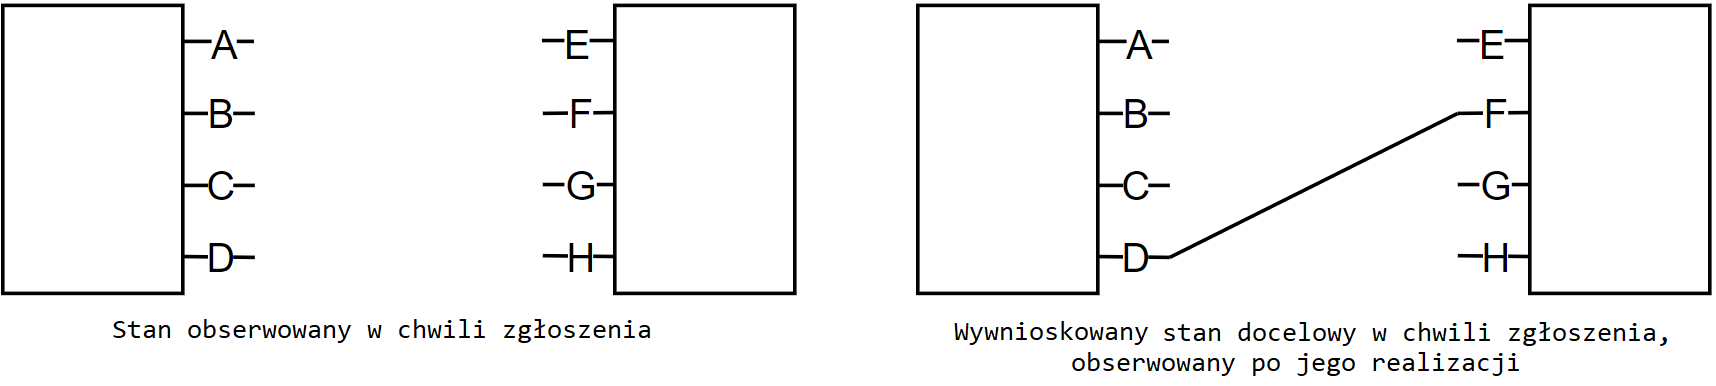
\includegraphics[width=1.0\linewidth]{22-system.png}
    \caption{Dwa stany systemu: sprzed, oraz po realizacji zgłoszenia o treści: "D" chce zadzwonić do "F"}\label{fig:}
\end{figure}

Pomówmy trochę o \hyperlink{def:wnioskowanie}{\textit{wnioskowaniu}}. Jak ono przebiega? Po pierwsze, telefonistka otrzymuje \hyperlink{def:dane}{\textit{dane}}. \textbf{Dane} to fakty lub statystyki zebrane w celu analizy. Telefonistka gromadzi dane w formie faktów dotyczących zaistniałych zdarzeń. Na przykład: dzwoni aparat telefoniczny, telefonistka podnosi słuchawkę i słyszy, że abonent chce połączyć się z abonentem mieszkającym w kamienicy pod numerem 35 na ulicy Polnej. Następnie dostępne dane zostają przekształcone w \hyperlink{def:informacja}{\textit{informację}}. \textbf{Informacja} to dane pozbawione formy przekazu. Równie dobrze rozmowa z abonentem mogłaby przebiec zupełnie inaczej, a telefonistka mogłaby otrzymać listowną prośbę o realizację połączenia. Różne dane mogą dostarczyć tę samą informację, czyli że abonent z określonego łącza chce dodzwonić się do abonenta z innego, konkretnego łącza. Gdy telefonistka uzyska informację o zgłoszeniu, łączy ją z posiadanymi już informacjami, np. dotyczącymi rozmieszczenia łączy na tablicy komutacyjnej. Następnie wykorzystuje swoją \hyperlink{def:wiedza}{\textit{wiedzę}}, czyli zestaw wzorców umożliwiających interpretację oraz przewidywanie tego, co się wydarzyło, co dzieje się obecnie i co może się wydarzyć w przyszłości. \textbf{Wiedza} opiera się na informacji oraz umiejętnościach zdobytych dzięki \hyperlink{def:doswiadczenie}{\textit{doświadczeniu}} lub \hyperlink{def:edukacja}{\textit{edukacji}}. Telefonistka obserwuje aktualny stan systemu i \hyperlink{def:wnioskowanie}{\textit{wnioskując}}, na podstawie wiedzy, wyobraża sobie stan docelowy (pożądany), a następnie definiuje akcje sterujące, które należy przeprowadzić na systemie, aby osiągnął on ten stan.


W przypadku komutacji proces wnioskowania jest stosunkowo prosty i możliwy do zapisania w języku programowania. Dlatego wraz z rozwojem technologicznym dokonano przejścia na automatyczne centrale telefoniczne. Jednak opisany powyżej schemat pozostaje aktualny. Do centrali trafiają dane w postaci sygnału na jednym z łączy. Sygnał zawiera numer MSISDN abonenta końcowego. Centrala przekształca te dane w informację, a następnie program w jej pamięci dokonuje wnioskowania. Wiedza potrzebna do wnioskowania zakodowana jest w programie. Dzięki programowalnym przełącznicom komutacyjnym również wykonanie akcji sterujacej (czyli połączenie dwóch łączy) jest możliwe bez udziału człowieka. 

W dzisiejszych czasach proces wnioskowania wykonywany przez ludzi nadzorujących systemy telekomunikacyjne nie jest już tak prosty. Dzięki wirtualizacji i programowalności funkcji sieciowych każdy rodzaj \hyperlink{def:wnioskowanie}{\textit{wnioskowania}}, który można sprowadzić do programu komputerowego, został już zautomatyzowany. Obecnie akcje wykonywane przez człowieka rzeczywiście wymagają jego inteligencji\footnote{lub sprawczości w świecie fizycznym, której komputerom brakuje}. Dlatego kolejnym etapem rozwoju telekomunikacji jest stworzenie inteligentnych sieci.